\documentclass{standalone}
\usepackage{tikz}
\usetikzlibrary{shapes,arrows.meta}
\begin{document}
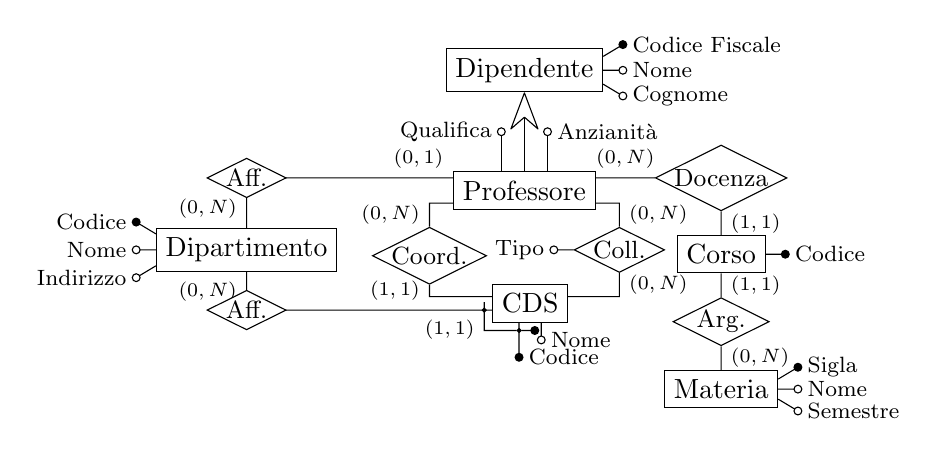
\begin{tikzpicture}
    \draw

    %%* Attributi:
    %%  node[draw, circle, inner sep=1pt, fill=black]{}node[right]{\footnotesize A}
    %%? Distanza orizzontale: E -(0.25,0.x)- A
    %%? Distanza verticale: E -(0,x * 0.22)- A

    %%* Cardinalità:
    %%  node[below right]{\scriptsize $(0,N)$}
    %%  node[above right]{\scriptsize $(0,N)$}
    %%  node[midway, above]{\scriptsize $(0,N)$}

    %%* Relazione:
    %%  node[draw, diamond, shape aspect=2, inner sep=3pt, anchor=90](r1){}
    %%  node[draw, diamond, shape aspect=2, inner sep=0.2pt, anchor=180](r2){R2}

    %%* Entità:
    %%  node[draw, rectangle, anchor=90](e1){}
    %%? Distanza verticale: E -(0.3)- R -(0.3) E
    %%? Distanza orizzontale: E -(0.75)- R -(0.75)- E

    %%* Professore
    (0,0)node[draw, rectangle, anchor=90](professore){Professore}
    (professore.40)--++(0,0.5)node[draw, circle, inner sep=1pt, fill=white]{}node[right]{\footnotesize Anzianità}
    (professore.140)--++(0,0.5)node[draw, circle, inner sep=1pt, fill=white]{}node[left]{\footnotesize Qualifica}

    ;
    %%* Dipendente
    \draw[-{Stealth[open, round, length=5mm]}](professore.90)--++(0,1)node[draw, rectangle, anchor=270](dipendente){Dipendente};\draw
    (dipendente.10)--++(0.25,0.15)  node[draw, circle, inner sep=1pt, fill=black]{}node[right]{\footnotesize Codice Fiscale}
    (dipendente.0)--++(0.25,0)      node[draw, circle, inner sep=1pt, fill=white]{}node[right]{\footnotesize Nome}
    (dipendente.350)--++(0.25,-0.15)node[draw, circle, inner sep=1pt, fill=white]{}node[right]{\footnotesize Cognome}

    %%* Corso
    (professore.10)--++(0.75,0)node[midway, above]{\scriptsize $(0,N)$}node[draw, diamond, shape aspect=2, inner sep=0.2pt, anchor=180](r1){\small Docenza}
    (r1.270)--++(0,-0.3)node[midway, right]{\scriptsize $(1,1)$}node[draw, rectangle, anchor=90](corso){Corso}
    (corso.0)--++(0.25,0)node[draw, circle, inner sep=1pt, fill=black]{}node[right]{\footnotesize Codice}


    %%* Materia
    (corso.270)--++(0,-0.3)node[midway, right]{\scriptsize $(1,1)$}node[draw, diamond, shape aspect=2, inner sep=0.2pt, anchor=90](r2){\small Arg.}
    (r2.270)--++(0,-0.3)node[midway, right]{\scriptsize $(0,N)$}node[draw, rectangle, anchor=90](materia){Materia}
    (materia.10)--++(0.25,0.15)  node[draw, circle, inner sep=1pt, fill=black]{}node[right]{\footnotesize Sigla}
    (materia.0)--++(0.25,0)      node[draw, circle, inner sep=1pt, fill=white]{}node[right]{\footnotesize Nome}
    (materia.350)--++(0.25,-0.15)node[draw, circle, inner sep=1pt, fill=white]{}node[right]{\footnotesize Semestre}


    %%* Corso di Studio
    (professore.350)--++(0.3,0)--++(0,-0.3)node[draw, diamond, shape aspect=2, inner sep=0.2pt, anchor=90](r3){\small Coll.}node[midway, right]{\scriptsize $(0,N)$}
    (r3.270)--++(0,-0.3)node[midway, right]{\scriptsize $(0,N)$}--++(-0.65,0)node[draw, rectangle, anchor=10](cds){CDS}
    (professore.190)--++(-0.3,0)--++(0,-0.3)node[draw, diamond, shape aspect=2, inner sep=0.2pt, anchor=90](r4){\small Coord.}node[midway, left]{\scriptsize $(0,N)$}
    (r4.270)--++(0,-0.15)node[midway, left]{\scriptsize $(1,1)$}-|(cds.170)
    (cds.240)--++(0,-0.1)node[draw, circle, inner sep=0.5pt, fill=black](b){}--++(0,-0.34)node[draw, circle, inner sep=1pt, fill=black]{}node[right]{\footnotesize Codice}
    (cds.300)--++(0,-0.22)node[draw, circle, inner sep=1pt, fill=white]{}node[right]{\footnotesize Nome}
    (r3.180)--++(-0.25,0)node[draw, circle, inner sep=1pt, fill=white]{}node[left]{\footnotesize Tipo}

    %%* Dipartimento
    (r3.180)++(-3,0)node[draw, rectangle, anchor=0](dip){Dipartimento}
    (dip.90)node[above left]{\scriptsize $(0,N)$}|-(professore.170)node[above left]{\scriptsize $(0,1)$}node[midway, draw, diamond, shape aspect=2, inner sep=0.2pt, fill=white](r5){\small Aff.}
    (dip.270)node[below left]{\scriptsize $(0,N)$}|-(cds.190)++(-0.1,0)node[below left]{\scriptsize $(1,1)$}node[draw, circle, inner sep=0.5pt, fill=black](a){}node[midway, draw, diamond, shape aspect=2, inner sep=0.2pt, fill=white](r6){\small Aff.}
    (dip.170)--++(-0.25,0.15) node[draw, circle, inner sep=1pt, fill=black]{}node[left]{\footnotesize Codice}
    (dip.180)--++(-0.25,0)    node[draw, circle, inner sep=1pt, fill=white]{}node[left]{\footnotesize Nome}
    (dip.190)--++(-0.25,-0.15)node[draw, circle, inner sep=1pt, fill=white]{}node[left]{\footnotesize Indirizzo}
    
    (a)++(0,0.1)|-(b)--++(0.2,0)node[draw, circle, inner sep=1pt, fill=black]{}


    ;
\end{tikzpicture}
\end{document}